\documentclass[10pt]{book}
\usepackage[text=17cm,left=2.5cm,right=2.5cm, headsep=20pt, top=2.5cm, bottom = 2cm,letterpaper,showframe = false]{geometry} %configuración página
\usepackage{latexsym,amsmath,amssymb,amsfonts} %(símbolos de la AMS).7
\parindent = 0cm  %sangria
\usepackage[T1]{fontenc} %acentos en español
\usepackage[spanish]{babel} %español capitulos y secciones
\usepackage{graphicx} %gráficos y figuras.

%---------------FORMATO de letra--------------------%

\usepackage{lmodern} % tipos de letras
\usepackage{titlesec} %formato de títulos
\usepackage[backref=page]{hyperref} %hipervinculos
\usepackage{multicol} %columnas
\usepackage{tcolorbox, empheq} %cajas
\usepackage{enumerate} %indice enumerado
\usepackage{marginnote}%notas en el margen
\tcbuselibrary{skins,breakable,listings,theorems}
\usepackage[Bjornstrup]{fncychap}%diseño de portada de capitulos
\usepackage[all]{xy}%flechas
\counterwithout{footnote}{chapter}
\usepackage{xcolor}
\usepackage[htt]{hyphenat}
%--------------------GRÀFICOS--------------------------

\usepackage{tkz-fct}

%---------------------------------

\titleformat*{\section}{\bfseries\rmfamily}
\titleformat*{\subsection}{\bfseries\rmfamily}
\titleformat*{\subsubsection}{\bfseries\rmfamily}
\titleformat*{\paragraph}{\bfseries\rmfamily}
\titleformat*{\subparagraph}{\bfseries\rmfamily}

%------------------------------------------

\renewcommand{\labelenumi}{\Roman{enumi}.}%primer piso II) enumerate
\renewcommand{\labelenumii}{\arabic{enumii}$)$}%segundo piso 2)
\renewcommand{\labelenumiii}{\alph{enumiii}$)$}%tercer piso a)
\renewcommand{\labelenumiv}{$\bullet$}%cuarto piso (punto)

%----------Formato título de capítulos-------------

\usepackage{titlesec}
\renewcommand{\thechapter}{\arabic{chapter}}
\titleformat{\chapter}[display]
{\titlerule[2pt]
\vspace{4ex}\bfseries\sffamily\huge}
{\filleft\Huge\thechapter}
{2ex}
{\filleft}

\begin{document}

\normalfont
\input xy
\xyoption{all}
\author{\Large Apuntes por FODE}
\title{\small Daniel M. Hausman \\ \vspace{1cm} \large La filosofía de la economía: Una ontología}
\date{}
\pagestyle{empty}
\maketitle
\thispagestyle{empty}
\let\cleardoublepage\clearpage
\tableofcontents								%indice





\begin{document}

    
    %----------caratula
    %\begin{titlingpage}

\newcommand\nbvspace[1][3]{\vspace*{\stretch{#1}}}
% allow some slack to avoid under/overfull boxes
\newcommand\nbstretchyspace{\spaceskip0.5em plus 0.25em minus 0.25em}
% To improve spacing on titlepages
\newcommand{\nbtitlestretch}{\spaceskip0.6em}
\pagestyle{empty}

\begin{center}
\bfseries
\nbvspace[1]

\Large Steven Brakman, Harry Garretsen, y Charles van Marrewijk\\
\Huge
{\nbtitlestretch\Huge LA NUEVA INTRODUCCIÓN A LA ECONOMÍA GEOGRÁFICA.}\\
\vspace{.5cm}
\large
\nbvspace[1]

APUNTES\\

\nbvspace[1]
\small POR\\
\Large FODE\\[0.5em]
\footnotesize CHRISTIAN LIMBERT PAREDES AGUILERA\\

\nbvspace[2]

\begin{center}
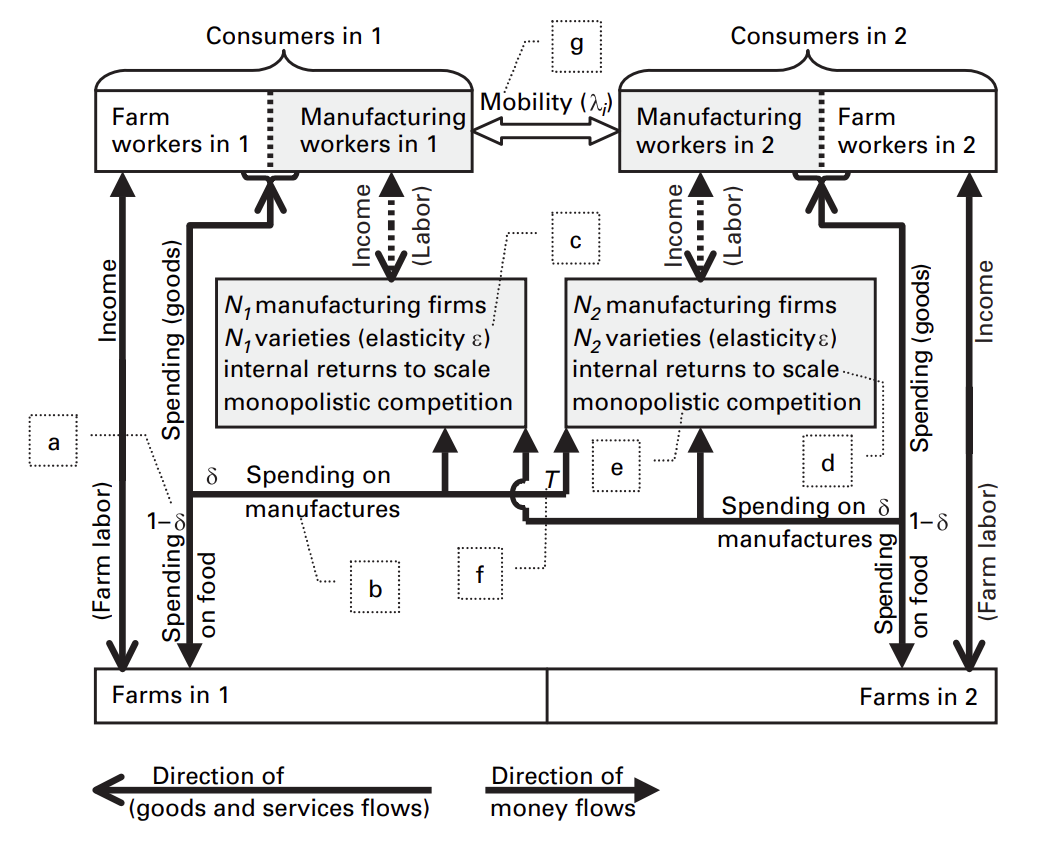
\includegraphics[scale=.3]{./imagen/diag.png}
\end{center}

\nbvspace[3]
\normalsize

LIBRO EN SU SEGUNDA EDICIÓN (Ingles)\\
\large
\nbvspace[1]

\end{center}

\break
\bfseries 

\nbvspace[1]
Título de la obra original:\\
THE NEW INTRODUCTION TO GEOGRAPHICAL ECONOMICS\\
Published in the United States of America by Cambridge University Press, New York\\

\nbvspace[1]

\begin{center}
Sin ninguna revisión de esta obra.\\


\nbvspace[1]
    Propiedad de esta obra:\\ 

    CHRISTIAN LIMBERT PAREDES AGUILERA\\	

    E-mail: soyfode@gmail.com
\end{center}

\nbvspace[1]

Reservados todos los derechos. La reproducción total o parcial de esta obra, por cualquier medio o procedimiento, comprendidos la reprografía y el tratamiento informático, y la distribución de ejemplares de ella mediante alquiler o préstamo públicos, queda rigurosamente prohibida sin la autorización escrita de los titulares del copyright, bajo las sanciones establecidas por las leyes.\\

\center 2022 

\end{titlingpage}


\pagenumbering{roman}

\tableofcontents								%indice

\pagestyle{fancy}
\fancyhead[LE,RO]{\nouppercase{\truncate{0.5\headwidth}{\rightmark}}}
\fancyhead[LO,RE]{\nouppercase{\truncate{0.5\headwidth}{\leftmark}}}



    
    %--------------------Estadística-------------------
	%----------tareas
	%% Options for packages loaded elsewhere
\PassOptionsToPackage{unicode}{hyperref}
\PassOptionsToPackage{hyphens}{url}
%
\documentclass[
]{article}
\usepackage{amsmath,amssymb}
\usepackage{iftex}
\ifPDFTeX
  \usepackage[T1]{fontenc}
  \usepackage[utf8]{inputenc}
  \usepackage{textcomp} % provide euro and other symbols
\else % if luatex or xetex
  \usepackage{unicode-math} % this also loads fontspec
  \defaultfontfeatures{Scale=MatchLowercase}
  \defaultfontfeatures[\rmfamily]{Ligatures=TeX,Scale=1}
\fi
\usepackage{lmodern}
\ifPDFTeX\else
  % xetex/luatex font selection
\fi
% Use upquote if available, for straight quotes in verbatim environments
\IfFileExists{upquote.sty}{\usepackage{upquote}}{}
\IfFileExists{microtype.sty}{% use microtype if available
  \usepackage[]{microtype}
  \UseMicrotypeSet[protrusion]{basicmath} % disable protrusion for tt fonts
}{}
\makeatletter
\@ifundefined{KOMAClassName}{% if non-KOMA class
  \IfFileExists{parskip.sty}{%
    \usepackage{parskip}
  }{% else
    \setlength{\parindent}{0pt}
    \setlength{\parskip}{6pt plus 2pt minus 1pt}}
}{% if KOMA class
  \KOMAoptions{parskip=half}}
\makeatother
\usepackage{xcolor}
\usepackage[margin=1in]{geometry}
\usepackage{graphicx}
\makeatletter
\def\maxwidth{\ifdim\Gin@nat@width>\linewidth\linewidth\else\Gin@nat@width\fi}
\def\maxheight{\ifdim\Gin@nat@height>\textheight\textheight\else\Gin@nat@height\fi}
\makeatother
% Scale images if necessary, so that they will not overflow the page
% margins by default, and it is still possible to overwrite the defaults
% using explicit options in \includegraphics[width, height, ...]{}
\setkeys{Gin}{width=\maxwidth,height=\maxheight,keepaspectratio}
% Set default figure placement to htbp
\makeatletter
\def\fps@figure{htbp}
\makeatother
\setlength{\emergencystretch}{3em} % prevent overfull lines
\providecommand{\tightlist}{%
  \setlength{\itemsep}{0pt}\setlength{\parskip}{0pt}}
\setcounter{secnumdepth}{-\maxdimen} % remove section numbering
\ifLuaTeX
  \usepackage{selnolig}  % disable illegal ligatures
\fi
\IfFileExists{bookmark.sty}{\usepackage{bookmark}}{\usepackage{hyperref}}
\IfFileExists{xurl.sty}{\usepackage{xurl}}{} % add URL line breaks if available
\urlstyle{same}
\hypersetup{
  pdftitle={Tarea 1},
  pdfauthor={Christian Limbert Paredes Aguilera},
  hidelinks,
  pdfcreator={LaTeX via pandoc}}

\title{Tarea 1}
\author{Christian Limbert Paredes Aguilera}
\date{2023-05-26}

\begin{document}
\maketitle

𝑝𝑝
\[\qquad w_{3t}^* = \dfrac{\mu_{3,t+1/t}/\sigma_{3,t+1/t}^2}{\dfrac{\mu_{1,t+1/t}^2}{\sigma_{1,t+1/t}}+\dfrac{\mu_{2,t+1/t}^2}{\sigma^2_{2,t+1/t}}+\dfrac{\mu_{3,t+1/t}^2}{\sigma^2_{3,t+1/t}}}\overline{\mu}_p,\]

\[\qquad w_{2t}^* = \dfrac{\mu_{2,t+1/t}/\sigma_{2,t+1/t}^2}{\dfrac{\mu_{1,t+1/t}^2}{\sigma_{1,t+1/t}}+\dfrac{\mu_{2,t+1/t}^2}{\sigma^2_{2,t+1/t}}+\dfrac{\mu_{3,t+1/t}^2}{\sigma^2_{3,t+1/t}}}\overline{\mu}_p,\qquad w_{3t}^* = \dfrac{\mu_{3,t+1/t}/\sigma_{3,t+1/t}^2}{\dfrac{\mu_{1,t+1/t}^2}{\sigma_{1,t+1/t}}+\dfrac{\mu_{2,t+1/t}^2}{\sigma^2_{2,t+1/t}}+\dfrac{\mu_{3,t+1/t}^2}{\sigma^2_{3,t+1/t}}}\overline{\mu}_p,\]

Elegimos 3 stock, Apple (AAPL) del sector tecnológico, NLY del sector
financiero(FCX) y Exxon Mobil Corporation XOM del sector del petróleo
para formar una cartera diversificada. La muestra consiste en precios
diarios desde el 2 de enero de 2008 hasta el 31 de mayo de 2013, para un
total de 1363 observaciones. Nos gustaría asignar el capital óptimamente
de tal modo que minimicemos el riesgo y obtengamos un rendimiento diario
medio de \(\overline{\mu}_p=0.15\) por ciento. Asumiendo que los stocks
en la cartera están incorrelacionados (sino a la varianza de la cartera
debería incorporarse los términos de covarianza), obtener las
ponderaciones óptimas siguiendo el problema de optimización planteado
anteriormente.

\begin{enumerate}
\def\labelenumi{\arabic{enumi}.}
\item
  Para ello en primer lugar, encontrar el mejor modelo para las series
  temporales de rendimientos de los 3 stocks tanto para la media
  condicional como para su varianza condicional.
\item
  Basándose en esos modelos obtener la media condicional y la varianza
  condicional y a partir de ellas calcular las ponderaciones óptimas
  variando en el tiempo.
\item
  Hacer gráficos de evolución temporal de esas ponderaciones e
  interpretarlos.
\item
  Realizar una tabla de los estadísticos descriptivos de las
  ponderaciones óptimas y comentarlos.
\end{enumerate}

\end{document}
 



    %--------------------Análisis de decisiones económicas y mercados----------------------
    %\chapter{Análisis de decisiones económicas y mercados}

\begin{multicols}{2}

\begin{itemize}
    \item Para criticar se debe conocer.
\end{itemize}

\section*{¿Qué preguntas puede abordar la teoría económica?.}

\begin{itemize}
    \item A la economía se le exige a más que otras ciencias. 
    \item ¿El objetivo de la ciencia en predecir?.
    \item El propósito de la ciencia es crear conocimiento donde se crea mundos abstractos.
\end{itemize}

    \subsection*{Objetivos de la economía}

    \begin{itemize}
	\item Entender el mundo real y,
	\item crear un lenguaje para poder discutir.
    \end{itemize}

    \subsection*{Métodos de investigación}
    \begin{itemize}
	\item Las ciencias físicas son mas fáciles que las ciencias económicas. Que sería si los electrones podrían pensar.
	\item Utilizamos el método inductivo.
    \end{itemize}

    \subsection*{¿Cual es el punto de partida para crear mundos abstractos?}
    Las llamamos las tres almas de Smith.
    \begin{enumerate}[1.]
	\item Estudiamos el comportamiento individual de los agentes.
	\item Un grupo es más que la suma de los individuos.
	\item Análisis de instituciones.
    \end{enumerate}
    \textbf{Se partirá del análisis individual}

    \subsection*{Los fundamentos de la escuela neoclásica}

    \begin{itemize}
	\item Se estudia ésta escuela porque es la mas exitosa hasta el momento.
	\item Se tiene tres características para poder ser identificado como neoclásico.
	\begin{enumerate}[1.]
	    \item Ser reduccionistas. Empezamos a analizar a los individuos.
	    \item ¿Que les motiva para tomar acciones?, los agentes deben ser racionales. 
	    \item Tener una noción de equilibro.
	\end{enumerate}
	\item No hay nada peor que estar adoctrinados y no saber lo que creemos.
	\item \textbf{Los economistas estudian decisiones, identificando factores que afectan esas decisiones y el resultado de la interacción de decisiones.}
    \end{itemize}




\end{multicols}

	
	%----------tareas

	    %tarea 4
		%\begin{enumerate}[\Large\bfseries 1.]

%--------------------1.--------------------
\item  \textbf{Construcción del agregado a partir de las decisiones individuales, y cálculo del equilibrio de mercado.} Se pide:

    \begin{enumerate}

	%----------1.a.
	\item[\bfseries 1.a]  \textbf{Construcción de la curvas de demanda de mercado.} Considere dos consumidores $i$ y $h$, donde sus respectivas curvas de demanda individuales de una mercancía son:


	donde sus respectivas curvas de demanda individuales de una mercancía son:
	$$q^i = d^i(p) = 21 - p$$ $$q^h = d^h(p) = 12-2p$$ 

	\begin{enumerate}[\bfseries i)]

		%----------i)
		\item Obtenga la \textbf{curva de demanda de mercado de un bien} $Q = D(p)$ como suma horizontal de las demandas individuales $(Q = D(p) \equiv d^i(p) + d^h(p))$\\\\
	    Respuesta.-\; $$Q = D(p) \equiv d^i(p) + d^h(p) = (21 - p) + (12 - 2p) = 33-3p$$\\

		%----------ii)
		\item Dibuje las curvas de demanda individuales, y la curva de demanda de mercado una al lado de la otra horizontalmente. En los tres gráficos indique las cantidades individuales y las de mercado que se consumen a un precio $p = 4$.

	    \end{enumerate}

	    \begin{multicols}{3}
		    \begin{center}
		    \begin{tikzpicture}[scale=.2]
			% abscisa y ordenada
			\tkzInit[xmax= 21,xmin=0,ymax=33,ymin=0]
			\tiny\tkzLabelXY[opacity=0.3,step=2, orig=false]
			% label x, f(x)
			\tkzDrawX[opacity= .6,label=p,right=0]
			\tkzDrawY[opacity= .6,label=$q^i$,below = -0.6]
			%dominio y función
			\draw [green,domain=0:21,thick,scale=1] plot(\x,{21-\x}); 
			\tkzText[red,above,opacity=1](10,32){\tiny $q^i = d^i(p)=21-p$}
			\draw[blue,dashed](4,0)--(4,17)--(0,17);
			\draw[blue](-2,17)node[left]{$q^i = 17$};
			\draw[blue](4,-2)node[below]{$p=4$};
		    \end{tikzpicture}
		    \end{center}

		    \begin{center}
		    \begin{tikzpicture}[scale=.2]
			% abscisa y ordenada
			\tkzInit[xmax=21,xmin=0,ymax=33,ymin=0]
			\tiny\tkzLabelXY[opacity=0.3,step=2, orig=false]
			% label x, f(x)
			\tkzDrawX[opacity= .6,label=p,right=0]
			\tkzDrawY[opacity= .6,label=$q^h$,below = -0.6]
			%dominio y función
			\draw [green,domain=0:6,thick,scale=1] plot(\x,{12-2*\x}); 
			\tkzText[red,above,opacity=1](10,32){\tiny $q^h = d^h(p) = 12-2p$}
			\draw[blue,dashed](4,0)--(4,4)--(0,4);
			\draw[blue](-1.5,4)node[left]{$q^i = 4$};
			\draw[blue](4,-2)node[below]{$p=4$};
		    \end{tikzpicture}
		    \end{center}

		    \begin{center}
		    \begin{tikzpicture}[scale=.2]
			% abscisa y ordenada
			\tkzInit[xmax= 21,xmin=0,ymax=33,ymin=0]
			\tiny\tkzLabelXY[opacity=0.3,step=2, orig=false]
			% label x, f(x)
			\tkzDrawX[opacity= .6,label=p,right=0]
			\tkzDrawY[opacity= .6,label=Q,below = -0.6]
			%dominio y función
			\draw [green,domain=0:11,thick,scale=1] plot(\x,{33-3*\x}); 
			\tkzText[red,above,opacity=1](10,32){\tiny $Q=D(p)=33-3p$}
			\draw[blue,dashed](4,0)--(4,21)--(0,21);
			\draw[blue](-2,21)node[left]{$q^i = 21$};
			\draw[blue](4,-2)node[below]{$p=4$};
		    \end{tikzpicture}
		    \end{center}
	    \end{multicols}
	    \vspace{.1cm}

	%----------1.b.
	\item[\bfseries 1.b.] \textbf{Construcción de la curvas de oferta de mercado.} Considere dos empresa, $j$ y $k$, donde sus respectivas ofertas individuales de una mercancía son:
	    $$q^j = o^j(p) = 5p-1$$ $$q^k = o^k(p) = p-2$$\\

	\begin{enumerate}[\bfseries i)]

		%----------i)
		\item Obtenga la \textbf{curva de oferta de mercado de un bien} $Q = D(p)$ como suma horizontal de las demandas individuales $(Q = O(p) \equiv o^j(p) + o^k(p))$\\\\
	    Respuesta.-\; $$Q = O(p) \equiv o^j(p) + o^k(p) = (5p-1) + (p-2) = 6p-3$$\\

		%----------ii)
		\item Dibuje las curvas de oferta individuales, y la curva de oferta de mercado una al lado de la otra horizontalmente. En los tres gráficos indique las cantidades individuales y las de mercado que se consumen a un precio $p = 4$.

	    \end{enumerate}

	    \begin{multicols}{3}
		    \begin{center}
		    \begin{tikzpicture}[scale=.2]
			% abscisa y ordenada
			\tkzInit[xmax= 19,xmin=0,ymax=33,ymin=0]
			\tiny\tkzLabelXY[opacity=0.3,step=2, orig=false]
			% label x, f(x)
			\tkzDrawX[opacity= .6,label=p,right=0]
			\tkzDrawY[opacity= .6,label=$q^i$,below = -0.6]
			%dominio y función
			\draw [green,domain=1/5:6,thick,scale=1] plot(\x,{5*\x-1}); 
			\tkzText[red,above,opacity=1](10,32){\tiny $q^j = o^j(p) = 5p-1$}
			\draw[blue,dashed](4,0)--(4,19)--(0,19);
			\draw[blue](-2,19)node[left]{$q^i = 19$};
			\draw[blue](4,-2)node[below]{$p=4$};
		    \end{tikzpicture}
		    \end{center}

		    \begin{center}
		    \begin{tikzpicture}[scale=.2]
			% abscisa y ordenada
			\tkzInit[xmax=19,xmin=0,ymax=33,ymin=0]
			\tiny\tkzLabelXY[opacity=0.3,step=2, orig=false]
			% label x, f(x)
			\tkzDrawX[opacity= .6,label=p,right=0]
			\tkzDrawY[opacity= .6,label=$q^h$,below = -0.6]
			%dominio y función
			\draw [green,domain=2:18,thick,scale=1] plot(\x,{\x-2}); 
			\tkzText[red,above,opacity=1](10,32){\tiny $q^k = o^k(p) = p-2$}
			\draw[blue,dashed](4,0)--(4,2)--(0,2);
			\draw[blue](-1.5,2)node[left]{$q^i = 2$};
			\draw[blue](4,-2)node[below]{$p=4$};
		    \end{tikzpicture}
		    \end{center}

		    \begin{center}
		    \begin{tikzpicture}[scale=.2]
			% abscisa y ordenada
			\tkzInit[xmax= 19,xmin=0,ymax=33,ymin=0]
			\tiny\tkzLabelXY[opacity=0.3,step=2, orig=false]
			% label x, f(x)
			\tkzDrawX[opacity= .6,label=p,right=0]
			\tkzDrawY[opacity= .6,label=Q,below = -0.6]
			%dominio y función
			\draw [green,domain=.5:5.5,thick,scale=1] plot(\x,{6*\x-3}); 
			\tkzText[red,above,opacity=1](10,32){\tiny $Q=O(p)=6p-3$}
			\draw[blue,dashed](4,0)--(4,21)--(0,21);
			\draw[blue](-2,21)node[left]{$q^i = 21$};
			\draw[blue](4,-2)node[below]{$p=4$};
		    \end{tikzpicture}
		    \end{center}
	    \end{multicols}
	    \vspace{.5cm}

	%----------1.c.
	\item[\bfseries 1.c.] Obtenga el equilibrio de mercado de la mercancía.\\\\
	    Respuesta.-\; Igualando la curva de oferta y demanda tenemos el precio de equilibrio,  $$33-3p=6p-3 \; \Longrightarrow \; p=4$$
	    luego obtenemos la cantidad de equilibro reemplazando $p$ en cualquiera de las curvas dadas, $$D(p)=33-4\cdot 4 \; \Longrightarrow \; D(p)=21$$\\ 
		    \begin{center}
		    \begin{tikzpicture}[scale=.2]
			% abscisa y ordenada
			\tkzInit[xmax= 19,xmin=0,ymax=33,ymin=0]
			\tiny\tkzLabelXY[opacity=0.3,step=2, orig=false]
			% label x, f(x)
			\tkzDrawX[opacity= .6,label=p,right=0]
			\tkzDrawY[opacity= .6,label=Q,below = -0.6]
			%dominio y función
			\draw [red,domain=.5:6,thick,scale=1] plot(\x,{6*\x-3}); 
			\tkzText[red,above,opacity=1](14,29){\tiny $Q=O(p)=6p-3$}
			\draw [green,domain=0:11,thick,scale=1] plot(\x,{33-3*\x}); 
			\tkzText[green,above,opacity=1](14,32){\tiny $Q=D(p)=33-3p$}
			\draw[blue,dashed](4,0)--(4,21)--(0,21);
			\draw[blue](-2,21)node[left]{$q^i = 21$};
			\draw[blue](4,-2)node[below]{$p=4$};
		    \end{tikzpicture}
		    \end{center}

    \end{enumerate}
\end{enumerate}


	    %tarea 5b
		%\subsection*{\center Ejercicio 5B. Teoría del consumidor}
\vspace{1cm}

\subsubsection*{\center I. Cálculo analítico de la función de demanda cuando la función de utilidad es diferenciable.}
\vspace{.5cm}


\begin{enumerate}[\large\bfseries 1.]

    %--------------------1.
    \item \textbf{¿Cómo calcular analíticamente la cesta óptima y la función de demanda cuando la función de utilidad es diferenciable.}\\\\
	Un consumidor, que posee una renta fija $\overline{M}[p.e., \overline{M} = 12]$, desea comprar dos mercancías que tienen un precio $(\overline{p_1} , \overline{p2})$. $[p.e., \overline{p} = (3, 1)]$. Las preferencias del consumidor sobre ambas mercancías están  representadas por la función de utilidad continua y diferenciable, $u(x1, x2) = x_1^\alpha x_2^\beta $ con $\alpha = \beta = 1$ (preferencias completas y monótonas).\\\\
Se pide:\\\\

    \begin{enumerate}[\bfseries a)]

	%----------a)
	\item \textbf{Función de demanda.} Suponga que el precio de las mercancías es $(p_1, p_2)$ y la renta del consumidor es $M$. Calcule analíticamente las funciones de demanda marshallianas;\\\\
	    Sea 

	%-----------b)
	\item \textbf{Elección óptima.} Calcule la cesta óptima para:\\\\ 

	    \begin{enumerate}[\bfseries b1)]

		%------b1
		\item Precios $\overline{p} = (\overline{p_1} , \overline{p_2} )=(3.00,1.00)$ y renta $\overline{M} =12$\\\\

		%------b2
		\item precios $\overline{p}^{'} = (\overline{p_1}^{'}, p_2 )=(12.00,1.00)$ y renta $\overline{M}=12$\\\

		%------b3
		\item precios $\overline{p}^{''} = (\overline{p_1}^{''} , p_2 )=(6.00,1.00)$ y renta $\overline{M} =12$.\\\\.

	    \end{enumerate}
	
	%----------c)
	\item Curvas de demanda. Represente gr´aficamente las curvas de demanda de los bienes 1 y
2 (respecto de sus precios), y sit´ue en las curvas de demanda las cestas ´optimas obtenidas
en b1)-b2)-b3) (Pista.- Recuerde la definici´on de curva de demanda, y tenga cuidado con los
desplazamientos de las curvas).\\\\
	
	%----------d)
	\item Función indirecta de utilidad. Calcule la función indirecta de utilidad.\\\\

    \end{enumerate}

\end{enumerate}


	    %tarea 5c 
		%\subsection*{\center Ejercicio 5C. Teoría del consumidor}
\vspace{1cm}

\subsubsection*{\center I. Describiendo los gustos individuales.}
\vspace{.5cm}

Invita a unos amigos a ver un partido en casa. Sus amigos quieren patatas fritas y cervezas, por lo que acude al supermercado donde existen dos tipos de mercancías: $‘$bolsas de patatas fritas$’$ (mercancía $1$) y $‘$latas de cerveza sueltas$’$ (mercancía $2$) (es decir, en el eje de abcisas vamos a indicar las patatillas y el de ordenadas las cervezas sueltas). En concreto, los gustos de sus amigos son tomar una bolsa de patatillas fritas por cada dos cervezas.\\\\

\begin{enumerate}[\large \bfseries 1.]

    %----------1.
    \item \textbf{¿Qué relación binaria caracteriza sus gustos con respecto a estas dos mercancías?}\\\\
	\textbf{Respuesta.-}\; En primer lugar el conjunto de consumo viene dado por las patatas fritas y las cervezas, es decir, $$\mathcal{X}^i = \lbrace x \in \mathbb{Z}^2 \; : \; x_l \geq 0 \; \mbox{para} \; l=1,2\rbrace.$$
	En segundo lugar, identificamos las cestas indiferentes. Por ejemplo, la cesta $"$bolsas de patatas fritas$"$ $\left( \mbox{cesta}\; (1,0) \right)$, es indiferente a la cesta $"$latas de cervezas sueltas$"$ $\left(\mbox{cesta}\; (0,2) \right)$, ya que, 
    $$\left.\begin{array}{rcl} (1,0)&\succeq&(0,2) \\ (0,2) & \succeq&(1,0) \end{array}\right\}\Longrightarrow (1,0) \sim (2,0)$$\\
	\begin{center}
	    \begin{tikzpicture}
		% abscisa y ordenada
		\tkzInit[xmax= 5.5,xmin=0,ymax=11,ymin=0,ystep=2]
		\tiny\tkzLabelX[opacity=0.4,step=1, orig=false]
		\tiny\tkzLabelY[opacity=0.4,step=1, orig=false]
		% label x, f(x)
		\tkzDrawX[opacity= 1,label=Patatas fritas , right=.5]
		\tkzDrawY[opacity= 1,label=Latas de cervezas, below = -.5]
		%dominio y función
		\draw[step=1cm,black,very thin,opacity=.1] (0,0) grid (6,6);
		\draw[color=red](1,0)--(0,1);
		\draw[color=red](2,0)--(0,2);
		\draw[color=red](3,0)--(0,3);
		\draw[color=red](4,0)--(0,4);
		\draw[color=red](5,0)--(0,5);

		\filldraw[black] (0,0)node[above right]{$(0,0)$} circle (1.5pt);

		\filldraw[black] (1,0)node[above right]{$(1,0)$} circle (1.5pt);
		\filldraw[black] (0,1)node[above right]{$(0,2)$} circle (1.5pt);

		\filldraw[black] (2,0)node[above right]{$(2,0)$} circle (1.5pt);
		\filldraw[black] (1,1)node[above right]{$(1,2)$} circle (1.5pt);
		\filldraw[black] (0,2)node[above right]{$(0,4)$} circle (1.5pt);

		\filldraw[black] (3,0)node[above right]{$(3,0)$} circle (1.5pt);
		\filldraw[black] (2,1)node[above right]{$(2,2)$} circle (1.5pt);
		\filldraw[black] (1,2)node[above right]{$(1,4)$} circle (1.5pt);
		\filldraw[black] (0,3)node[above right]{$(0,6)$} circle (1.5pt);

		\filldraw[black] (4,0)node[above right]{$(4,0)$} circle (1.5pt);
		\filldraw[black] (3,1)node[above right]{$(3,1)$} circle (1.5pt);
		\filldraw[black] (2,2)node[above right]{$(2,4)$} circle (1.5pt);
		\filldraw[black] (1,3)node[above right]{$(1,6)$} circle (1.5pt);
		\filldraw[black] (0,4)node[above right]{$(0,8)$} circle (1.5pt);

		\filldraw[black] (5,0)node[above right]{$(5,0)$} circle (1.5pt);
		\filldraw[black] (4,1)node[above right]{$(4,2)$} circle (1.5pt);
		\filldraw[black] (3,2)node[above right]{$(3,4)$} circle (1.5pt);
		\filldraw[black] (2,3)node[above right]{$(2,6)$} circle (1.5pt);
		\filldraw[black] (1,4)node[above right]{$(1,8)$} circle (1.5pt);
		\filldraw[black] (0,5)node[above right]{$(0,10)$} circle (1.5pt);
	    \end{tikzpicture}
	\end{center}
	\vspace{.5cm}

	Análogamente la cesta $(2,0)$ es indiferente a las cestas $(0,4)$ y $(1,2)$, como también la cesta $(3,0)$ es indiferente a las cestas $(0,6),\; (1,4)$ y $(2,2)$. Por lo tanto una cesta $x=(x_1,x_2)$ es indiferente a otra $y=(y_1,y_2)$ si, $$2x_1 + x_2 = 2y_1 + y_2.$$
	Por último caracterizamos formalmente los gustos a través de la relación binaria $"$ser como mínimo tan preferido como$"$ como sigue,
	\begin{center}
	    Dado cualquier par de cestas $x,y \in \mathcal{X}^i$ entonces $x \succeq^i y \; \Longleftrightarrow 2x_1 + x_2 \geq 2y_1 + y_2$.
	\end{center}
	\vspace{.5cm}

    %----------2.
    \item \textbf{¿Puede representar sus gustos a través de conjuntos de indiferencia?}\\

	\begin{enumerate}[\bfseries (2.1)]

	    %----------(2.1)
	    \item Siendo que cumplen los axiomas de completitud y transitividad, tenemos que,
		$$x,y\in \mathcal{X}^i \; \mbox{entonces} \; x\succeq^i y \; \Longleftrightarrow \; 2x_1+x_2 \geq 2y_1+y_2.$$
		Luego y sabiendo que las ordenaciones serán consistente, es decir, que podemos identificar conjuntos de cestas indiferentes, podemos definirlas como, 
		$$\mathcal{I}^i(x) = \lbrace y\in \mathcal{X}^i\; : \;  2x_1 + x_2 = 2y_1 + y_2\rbrace.$$
		Y por lo tanto, los gustos están representados por $\left(\mathcal{X}^i,\lbrace \mathcal{I}^i(x)\rbrace_{x\in \mathcal{X}^i}\right)$. Por ejemplo, ya que $2\cdot 1 + 0 = 2\cdot 0 + 2$ entonces,
		$$\mathcal{I}^i (1,0) = \lbrace (0,2) \rbrace$$
		
		\begin{center}
		    \begin{tikzpicture}
			% abscisa y ordenada
			\tkzInit[xmax= 5,xmin=0,ymax=10,ymin=0,ystep=2]
			\tiny\tkzLabelX[opacity=0.4,step=1, orig=false]
			\tiny\tkzLabelY[opacity=0.4,step=1, orig=false]
			% label x, f(x)
			\tkzDrawX[opacity= 1,label=Patatas fritas , right=.5]
			\tkzDrawY[opacity= 1,label=Latas de cervezas, below = -.5]
			%dominio y función
			\draw[step=1cm,black,very thin,opacity=.1] (0,0) grid (5,5);
			\draw[color=red](1,0)--(0,1);
			\draw[color=red](2,0)--(0,2);
			\draw[color=red](3,0)--(0,3);
			\draw[color=red](4,0)--(0,4);
			\draw[color=red](5,0)--(0,5);
			\draw[opacity=.7](-.1,0)node[above right]{$\mathcal{I}_a$};
			\draw[opacity=.7](.4,.5)node[above right]{$\mathcal{I}_b$};
			\draw[opacity=.7](.9,1)node[above right]{$\mathcal{I}_c$};
			\draw[opacity=.7](1.4,1.5)node[above right]{$\mathcal{I}_d$};
			\draw[opacity=.7](1.9,2)node[above right]{$\mathcal{I}_e$};
			\draw[opacity=.7](2.4,2.5)node[above right]{$\mathcal{I}_f$};
		    \end{tikzpicture}
		\end{center}
		\vspace{.5cm}

		De manera similar $$\mathcal{I}^i(2,0) = \lbrace (1,2),(0,4) \rbrace \quad;\quad \mathcal{I}^i(3,0) = \lbrace (2,2),(1,4),(0,6) \rbrace \quad ...$$\\

	    %----------(2.2)
	    \item El gráfico de conjuntos indiferentes para $(1,2)$, $(2,4)$ y $(3,6)$ esta dado por

		\begin{center}

		    \begin{tikzpicture}
			% abscisa y ordenada
			\tkzInit[xmax= 6,xmin=0,ymax=12,ymin=0,ystep=2]
			\tiny\tkzLabelX[opacity=0.4,step=1, orig=false]
			\tiny\tkzLabelY[opacity=0.4,step=1, orig=false]
			% label x, f(x)
			\tkzDrawX[opacity= 1,label=Patatas fritas , right=.5]
			\tkzDrawY[opacity= 1,label=Latas de cervezas, below = -.5]
			%dominio y función
			\draw[step=1cm,black,very thin,opacity=.1] (0,0) grid (6,6);
			\draw[color=red](2,0)--(0,2);
			\draw[color=red](4,0)--(0,4);
			\draw[color=red](6,0)--(0,6);

			\filldraw[black] (2,0)node[above right]{$(2,0)$} circle (1.5pt);
			\filldraw[red] (1,1)node[above right]{$\mathcal{I}^i(1,2)$} circle (1.5pt);
			\filldraw[black] (0,2)node[above right]{$(0,4)$} circle (1.5pt);

			\filldraw[black] (4,0)node[above right]{$(4,0)$} circle (1.5pt);
			\filldraw[black] (3,1)node[above right]{$(3,1)$} circle (1.5pt);
			\filldraw[red] (2,2)node[above right]{$\mathcal{I}^i(2,4)$} circle (1.5pt);
			\filldraw[black] (1,3)node[above right]{$(1,6)$} circle (1.5pt);
			\filldraw[black] (0,4)node[above right]{$(0,8)$} circle (1.5pt);

			\filldraw[black] (6,0)node[above right]{$(6,0)$} circle (1.5pt);
			\filldraw[black] (5,1)node[above right]{$(5,1)$} circle (1.5pt);
			\filldraw[black] (4,2)node[above right]{$(4,4)$} circle (1.5pt);
			\filldraw[red] (3,3)node[above right]{$\mathcal{I}^i(3,6)$} circle (1.5pt);
			\filldraw[black] (2,4)node[above right]{$(2,8)$} circle (1.5pt);
			\filldraw[black] (1,5)node[above right]{$(1,10)$} circle (1.5pt);
			\filldraw[black] (0,6)node[above right]{$(0,12)$} circle (1.5pt);
		    \end{tikzpicture}

		    $\begin{tabular}{rcl}
			$\mathcal{I}^i(1,2)$&$=$&$\lbrace (0,4),(2,0) \rbrace$\\\\
			$\mathcal{I}^i(2,4)$&$=$&$\lbrace (0,8),(1,6),(3,1),(4,0)\rbrace$\\\\
			$\mathcal{I}^i(3,6)$&$=$&$\lbrace (0,12),(1,10),(2,8),(4,4),(5,1),(6,0) \rbrace$\\
		    \end{tabular}$\\
    
		\end{center}
		\vspace{.5cm}

	    %----------(2.3)
	    \item Sabiendo que la relación marginal de sustitución es lo máximo que estaría dispuesto a renunciar para consumir otra mercancía (pendiente de la curva de indiferencia), entonces la $RMS$ de consumir una $"$bolsa patatas fritas$"$ estaría dado por $2$ $"$latas de cervezas$"$, es decir, 
		$$MRS(patatas) = 2.$$
		En su defecto podríamos decidir consumir una $"$lata de cerveza$"$ más, entonces la $RMS$ estará dado por  media bolsa de $"$patatas fritas$"$, es decir,
		$$MRS(cerveza) = \dfrac{1}{2}.$$
		Con el único inconveniente que no podemos que no podemos eligir media bolsa de patatas fritas.\\\\

	\end{enumerate}

    %--------------------3.
    \item \textbf{¿Puede representar sus gustos a través de una función de utilidad?}\\

	\begin{enumerate}[\bfseries (3.1)]
	    %----------(3.1)
	    \item Para tal efecto necesitamos que a cada cesta se le asigne un número real de tal forma que se cumple el criterio de que si una cesta es indiferente a una segunda entonces le daremos el mismo valor numérico y si una cesta es estrictamente mas preferida que una tercera entonces se dará valores distintos. Se representa de la siguiente manera:     
		\begin{center}
		    \begin{tabular}{rccc|ccc}
			$u:$&$\mathcal{X}$ & $\longmapsto$ & $\mathbb{R}$ & $x \sim y$ & $\Rightarrow$ & $u(x)=u(y)$\\
			    & $x$ & $\longmapsto$ & $u(x_1,x_2)$ & $x\succ z$&$\Rightarrow$&$u(x)>u(z)$\\
		    \end{tabular}
		\end{center}
		\vspace{.3cm}
		Luego podríamos asignar dicha función de utilidad en función a la cantidad total de cervezas. 
		$$u(x_1,x_2)=2x_1+x_2$$
		Por ejemplo

		\begin{center}
		    \begin{tabular}{cccccc}
			$u:$&$\mathcal{X}$&$\longmapsto$&$\mathbb{R}$&&\\
			 & $(x_1,x_2)$ & $\longmapsto$&$u(x_1,x_2)$&$=$&$2x_1+x_2$\\
			    & $(0,0)$ & $\longmapsto$ & $u(0,0)$ & $=$ & $0$\\
			    & $(1,0)$ & $\longmapsto$ & $u(1,0)$ & $=$ & $2$\\
			    & $(0,2)$ & $\longmapsto$ & $u(0,2)$ & $=$ & $2$\\
			    & $(2,0)$ & $\longmapsto$ & $u(2,0)$ & $=$ & $4$\\
			    & $(1,2)$ & $\longmapsto$ & $u(1,2)$ & $=$ & $4$\\
			    & $(0,4)$ & $\longmapsto$ & $u(0,4)$ & $=$ & $4$\\
			    & $(3,0)$ & $\longmapsto$ & $u(3,0)$ & $=$ & $6$\\
			    & $(2,2)$ & $\longmapsto$ & $u(2,2)$ & $=$ & $6$\\
			    & $(1,4)$ & $\longmapsto$ & $u(1,4)$ & $=$ & $6$\\
			    & $(0,6)$ & $\longmapsto$ & $u(0,6)$ & $=$ & $6$\\
		    \end{tabular}
		\end{center} 
		\vspace{.6cm}

		%----------(3.2)
		\item Anteriormente para los cardinalistas, la función de utilidad que representaba las preferencias de un consumidor era única y  la representación de los gustos individuales de un consumidor en la teoría económica moderna es ordinalista es decir, se representan a través de una representación binaria que ordena cestas . Acá la cuestión es si existe una relación entre la herramienta de los cardinalistas (la función de utilidad) y la herramienta de los ordinalistas (relación de preferencias). \\
Dicho esto nos preguntamos que si para una representación de gustos a través de una relación de preferencias, existe una única función de utilidad o pueden existir más de una?. \\ 
A pesar del hecho que para los cardinalistas la función de preferencias de un consumidor era única, esta desapareció, por lo tanto la respuesta a esta cuestión es que no existe una única función de utilidad, es más existen infinitas funciones de utilidad, esto ya que al asignar números reales a cada preferencia, solo las asignamos por un propósito de ordenación que solo representan los gustos. \\\\

	    \end{enumerate}


\subsubsection*{\center II. Elección óptima.}
\vspace{.5cm}

    %-------------------4.
    \item \textbf{¿Cuál es la decisión óptima?.}\\\\
	Sus amigos han reunido $\overline{M} =12 \EUR$ (la renta). El precio de las patatillas fritas son $p_1 =1 \EUR$ y el de las cervezas sueltas es $p_2 =1 \EUR$; es decir, 
	$p = (p_1 , p_2 ) =$ $(1.00 \EUR$,  $1.00 \EUR $).\\

	\begin{enumerate}[\bfseries (4.1)]

	    %----------(4.1)
	    \item Sabiendo que los gustos de mis amigos son tomar una bolsa de patatas fritas por cada dos cervezas, entonces la cesta que elegiría sería la $(4,8)$, ya que querrán comer lo máximo en patatas como también cerveza en función a las preferencias mencionadas.\\\\ 

	    %----------(4.2)
	    \item El conjunto de consumo como sabemos esta dado por,
		$$\mathcal{X} = \lbrace (p,c) \; /\; p,c > 0\rbrace,$$
		luego la renta y los precios están  dados por,
		\begin{center} $\overline{M} = 12 \EUR$ , $\qquad (\overline{p_1},\overline{p_2}) = (1,1)$, \end{center}
		por último el conjunto presupuestario será,
		$$\beta(\overline{p_1},\overline{p_2},\overline{M}) = \lbrace (p,c) \in \mathcal{X} \; /\; \overline{p_1}\cdot p + \overline{p_2}\cdot c \leq \overline{M}\rbrace.$$
		\vspace{.1 cm}

		\begin{center}
		    \begin{tikzpicture}[scale=.9]
			% abscisa y ordenada
			\tkzInit[xmax= 12.5,xmin=0,ymax=25,ymin=0,ystep=2]
			\tiny\tkzLabelX[opacity=0.4,step=1, orig=false]
			\tiny\tkzLabelY[opacity=0.4,step=1, orig=false]
			% label x, f(x)
			\tkzDrawX[opacity= 1,label=Patatas fritas (p), right=.1]
			\tkzDrawY[opacity= 1,label=Latas de cervezas (c), below = -.5]
			%dominio y función
			\draw[step=1cm,black,very thin,opacity=.03] (0,0) grid (12,12);
			\draw[opacity = 0.1,color=red](1,0)--(0,1);
			\draw[opacity = 0.1,color=red](2,0)--(0,2);
			\draw[opacity = 0.1,color=red](3,0)--(0,3);
			\draw[opacity = 0.1,color=red](4,0)--(0,4);
			\draw[opacity = 0.1,color=red](5,0)--(0,5);
			\draw[opacity = 0.1,color=red](6,0)--(0,6);
			\draw[opacity = 0.1,color=red](7,0)--(0,7);
			\draw[opacity = 0.1,color=red](8,0)--(0,8);
			\draw[opacity = 0.1,color=red](9,0)--(0,9);
			\draw[opacity = 0.1,color=red](10,0)--(0,10);
			\draw[opacity = 0.1,color=red](11,0)--(0,11);
			\draw[opacity = 0.1,color=red](12,0)--(0,12);
			\draw[opacity = 1,color=blue](12,0)--(0,6);

			\draw[blue](12,-1)node[]{$\left(\frac{\overline{M}}{\overline{p_1}},0\right)\equiv (12,0)$};
			\draw[blue](-1.8,6)node[]{$\left(0,\frac{\overline{M}}{\overline{p_2}}\right)\equiv (0,12)$};

			\filldraw[black] (1,6)node[above]{$(1,12)$} circle (1.5pt);
			\filldraw[green] (1,5)node[below]{$(1,10)$} circle (1.5pt);
			\filldraw[red] (1,5.5)node[above right]{$(1,11)$} circle (1.5pt);

			\draw[green,dashed](1,6)--(1,5);
			\draw[green, dashed](0,6)--(1,6);
			\draw[green, dashed](0,5)--(1,5);
			\draw[green, <->, dashed](-0.6,5)--(-0.6,6);
			\draw[green](-1,5.5)node[]{$RMS$};

			\draw[red,dashed](1,6)--(2.5,6)--(2.5,5.5)--(1,5.5);
			\draw[red, <->, dashed](2.8,5.5)--(2.8,6);
			\draw[red](3.3,5.75)node[]{$RMI$};

			\draw[green,dashed](1,5.5)--(2,5.5);
			\filldraw(2,5.5)node[below right]{$(2,11)$} circle (1.5pt);

		    \end{tikzpicture}
		\end{center}
		\vspace{.5cm}

		    Suponiendo que primero nos encontramos con el anaquel de las latas sueltas entonces nos preguntaremos..\\

		\begin{enumerate}[1.-]

		    \item (0,12) ¿Debo meter una bolsa de patatas fritas en el carro?\\\\
			Para ello aplicamos la regla de decisión racional como también la relación marginal de sustitución $(RMS)$ y la relación marginal de intercambio $RMI = \dfrac{\overline{p_1}}{\overline{p_2}}$\\
			\begin{center}
			    \begin{tabular}{rcccccl}
				&&$B(p)$&$>$&$C(p)$&&\\\\
				\hline\\
				$RMS$ & $=$ & $2$ & $>$ & $1$ & $=$ & $RMI$\\\\
			    \end{tabular}
		    \end{center}

		    \item (1,11)

		\end{enumerate}

	\end{enumerate}

\subsubsection*{\center III. Curva de demanda.}
\vspace{.5cm}

    %--------------------5.
    \item ¿Cómo vería la decisión óptima cuando se modifica el conjunto presupuestario (cambios en precios o renta)?


\subsubsection*{\center IV. Cálculo analítico de la función de demanda.}
\vspace{.5cm}

    %--------------------6.
    \item ¿Cómo calcular analíticamente la cesta óptima y la función de demanda?\\\\
	Suponga que las preferencias de un consumidor están representadas por la función de utilidad continua $u(x_1, x_2) = min\lbrace2x_1, x_2\rbrace$. Se pide:

	\begin{enumerate}[\bfseries a)]

	    %---------- a)
	    \item \textbf{Función de demanda.} Suponga que el precio de las mercancías es $(p_1, p_2)$ y la renta del consumidor es $M$. Calcule analíticamente las funciones de demanda marshallianas;\\\\
		\textbf{Respuesta.-}\; Sean el conjunto de consumo, $$\mathcal{X} = \lbrace (x_1,x_2 \; / \; p \geq 0, c\geq 0 \rbrace,$$
		el conjunto presupuestario, $$\lbrace(x_1,x_2)\in \mathcal{X} \; / \; \overline{p_1}x_1 + \overline{p_2} x_2 \leq \overline{M}\rbrace,$$
		y la función de utilidad $$u(x_1,x_2) = min\lbrace2x_1,x_2\rbrace$$
		entonces, el problema de consumidor estará dado por:
		$$\left\{\begin{array}{ccc}
			\max\limits_{x_1,x_2}&&u(x_1,x_2)=min\lbrace2x_1,x_2\rbrace\\\\
					     &s.a.&\begin{array}{rcl} \overline{p_1}x_1 + \overline{p_2}x_2&\leq &\overline{M}\\ x_1&\leq&0\\ x_2&\geq & 0 \end{array}\\\\
			   &dado&\overline{p_1},\overline{p_2},\overline{M}\\
		\end{array}\right.$$

	\end{enumerate}

	y sabiendo que las preferencias son monótonas con lo que $$\overline{p_1}x_1+\overline{p_2}x_2=\overline{M}\; \Longrightarrow \; x_2 = \dfrac{\overline{M}}{\overline{p_2}}-\dfrac{\overline{p_1}}{\overline{p_2}}x_1$$ de donde sustituyéndolo en la función de utilidad nos queda,
	$$\theta(x_1) = min\lbrace$$


\end{enumerate}


	    %tarea 6
		%\subsection*{\center Ejercicio 6. Teoría de la Empresa}
\vspace{1cm}

\begin{enumerate}[\large\bfseries 1.]

    %--------------------1.
    \item \textbf{Asignación de un recurso entre dos actividades}\\\\
    
    \begin{tcolorbox}[colframe=white]
	\begin{center}
	    \begin{tabular}{||ccc||c||ccc||}
		\hline
		$ProdMarg_O$&$PromProd_O$&$q_O$ (Tm)&Flota&$q_E$(Tm)&$PromProd_E$&$ProdMarg_E$\\	
		\hline
		 0&0&0&0&0&0&0\\
		 100&100&100&1&130&130&130\\
		 100&100&200&2&240&120&110\\
		 100&100&300&3&330&110&90\\
		 80&85&380&4&400&100&70\\
		 \hline
	    \end{tabular}
	\end{center}
    \end{tcolorbox}

	\begin{multicols}{2}
	    \begin{center}
		\begin{tikzpicture}[scale=1.15]
		    % abscisa y ordenada
		    \tkzInit[xmax= 5,xmin=0,ymax=500,ymin=0,ystep=100]
		    \tiny\tkzLabelX[opacity=0.4,step=1, orig=false]
		    \tiny\tkzLabelY[opacity=0.4,step=1, orig=false]
		    % label x, f(x)
		    \tkzDrawX[opacity= 1,label=Labor, right=.1]
		    \tkzDrawY[opacity= 1,label=Produción, below = -.5]
		    %dominio y función
		    \draw[step=1cm,black,very thin,opacity=.05] (0,0) grid (5.5,5.5);
		    \filldraw[black](0,0)node[below left]{$(0,0)$} circle (1.5pt);

		    \node at (2.5,6.5) {\textbf{Curvas de producto total, marginal y medio (E)}};

		    \filldraw[red](1,1.3)node[left]{$(1,130)$} circle (1.5pt);
		    \filldraw[red](2,1.1)node[below left]{$(2,110)$} circle (1.5pt);
		    \filldraw[red](3,0.9)node[below left]{$(3,90)$} circle (1.5pt);
		    \filldraw[red](4,0.7)node[below left]{$(4,70)$} circle (1.5pt);

		    \draw[red](0,0)..controls(1,1.55)..(2,1.1);
		    \draw[red](2,1.1)..controls(3,.9)..(4,0.7)node[below right]{$ProdMarg_E$};

		    \filldraw[green](2,2.4)node[above left]{$(2,240)$} circle (1.5pt);
		    \filldraw[green](3,3.3)node[above left]{$(3,330)$} circle (1.5pt);
		    \filldraw[green](4,4)node[above left]{$(4,400)$} circle (1.5pt);

		    \draw[green](0,0)..controls(1.3,2)and(3.5,4)..(5,4.5);
		    \draw[green](5.1,4.6)node[above]{$Producción E$};


		    \filldraw[blue](1,1.3)node[above right]{$(1,130)$} circle (1.5pt);
		    \filldraw[blue](2,1.2)node[above right]{$(2,120)$} circle (1.5pt);
		    \filldraw[blue](3,1.1)node[above right]{$(3,110)$} circle (1.5pt);
		    \filldraw[blue](4,1)node[above right]{$(4,100)$} circle (1.5pt);

		    \draw[blue](0,0)..controls(1,1.5)..(2,1.2);
		    \draw[blue](2,1.2)..controls(3,1.1)..(4,1)node[below right]{$PromProd_E$};
		    \draw[blue](5.1,4.25);
		\end{tikzpicture}
	    \end{center}

	    \begin{center}
		\begin{tikzpicture}[scale=1.15]
		    % abscisa y ordenada
		    \tkzInit[xmax= 5,xmin=0,ymax=500,ymin=0,ystep=100]
		    \tiny\tkzLabelX[opacity=0.4,step=1, orig=false]
		    \tiny\tkzLabelY[opacity=0.4,step=1, orig=false]
		    % label x, f(x)
		    \tkzDrawX[opacity= 1,label=Labor, right=.1]
		    \tkzDrawY[opacity= 1,label=Produción, below = -.5]
		    %dominio y función
		    \draw[step=1cm,black,very thin,opacity=.05] (0,0) grid (5.5,5.5);

		    \node at (2.5,6.5) {\textbf{Curvas de producto total, marginal y medio (O)}};

		    \filldraw[black](0,0)node[below left]{$(0,0)$} circle (1.5pt);

		    \filldraw[red](1,1)node[left]{$(1,100)$} circle (1.5pt);
		    \filldraw[red](2,1)node[below left]{$(2,100)$} circle (1.5pt);
		    \filldraw[red](3,1)node[below left]{$(3,100)$} circle (1.5pt);
		    \filldraw[red](4,.8)node[below left]{$(4,80)$} circle (1.5pt);

		    \draw[red](0,0)..controls(1,1.2)..(2,1);
		    \draw[red](2,1)..controls(3,1.05)..(4,.8)node[below right]{$ProdMarg_O$};

		    \filldraw[green](2,2)node[below right]{$(2,200)$} circle (1.5pt);
		    \filldraw[green](3,3)node[below right]{$(3,300)$} circle (1.5pt);
		    \filldraw[green](4,3.8)node[below right]{$(4,380)$} circle (1.5pt);

		    \draw[green](0,0)..controls(1.9,1.75)and(3,3.5)..(5,4.3);
		    \draw[green](5.1,4.48)node[above]{$Producción O$};

		    \filldraw[blue](2,1)node[above]{$(2,100)$} circle (1.5pt);
		    \filldraw[blue](3,1)node[above]{$(3,100)$} circle (1.5pt);
		    \filldraw[blue](4,.85)node[above]{$(4,85)$} circle (1.5pt);

		    \draw[blue,opacity=.7](0,0)..controls(1,1.2)..(2,1);
		    \draw[blue,opacity=.7](2,1)..controls(3,1.05)..(4,.85)node[right]{$PromProd_O$};
		    \draw[blue](5.1,4.25);
		\end{tikzpicture}
	    \end{center}
	\end{multicols}
	    \vspace{1cm}

	\begin{enumerate}[\bfseries a)]

	    %----------a)
	    \item Utilizando la teoría económica, explíquele a su armador cuál es la distribución óptima entre ambos bancos de pesca.\\\\
		A pesar de que los gráficos nos dan un panorama general, analizaremos en particular los barcos, como recursos que no son perfectamente divisibles. La teoría económica es la siguiente:
		\begin{center}
		    $"$ Para repartir eficientemente un recurso entre diferentes actividades productivas consiste en asignar cada unidad del recurso a la actividad productiva en la que su producto marginal es el más alto  (Robert Frank) $"$.
		\end{center}
		Ahora bien para hallar la distribución óptima entre los dos barcos de pesca simplemente se deducirá a la mayor distribución de su producción total, en este caso 440 toneladas (100 de cada uno de los barcos del Oeste y 120 de los barcos del lado Este.) como se verá en la siguiente tabla.\\\\
	    \begin{tcolorbox}[colframe=white]
		\begin{center}
		    \begin{tabular}{|cc||c|}
			\hline
			barco Este&Barco Oeste&cantidades producidas\\
			\hline
			4&0&400\\
			3&1&430\\
			\hline
			2&2&440\\
			\hline
			1&3&430\\
			0&4&380\\
			\hline
		    \end{tabular}
		\end{center}
	    \end{tcolorbox}
	    \vspace{1cm}

	    %---------b)
	    \item Hágale ver cuál es su error al tomar la productividad media tanto al principio cuando quería mandar todos los barcos hacia Rande, como después que quería mandar un barco más a Rande.\\\\
	    Sabiendo que los costes de mandar a cualquiera de los dos bancos de pesca son iguales , Supongamos que mandamos solamente dos barcos hacia Rande, por lo tanto la captura media estará dado por 20 toneladas diarias, más que las capturas del otro extremo. A esto observe que si mandamos un tercer barco a Rande, la contribución a la cantidad total será de 90 toneladas, es decir, la diferencia entre 330 Toneladas y 240 Toneladas. Algo muy importante es el hecho de que el tercer barco que pesta en Rande captura del pescado que habría sido capturado por los dos primeros.\\
Por lo tanto el coste de oportunidad de mandar un tercer barco a Rande son las 100 toneladas que ya no se capturaran en las Islas Cíes, como se verá a continuación:\\

    	    \begin{tcolorbox}[colframe=white]
	    \begin{center}
		\begin{tabular}{ccc}
		    B(Rande)&>&C(Istas Cíes)\\
		    \hline
		    90&$\ngtr$&100\\
		\end{tabular}
	    \end{center}
	    \end{tcolorbox}
	    Análogamente, si enviamos un cuarto barco a Rande, el coste de oportunidad será de $100$  y el beneficio solo de 70 toneladas.\\\\

	\end{enumerate}

    %--------------------2.
    \item \textbf{La decisión de producción de la empresa basadas en la productividad de los inputs productivos deben coincidir con la decisión de producción de la empresa basadas en los costes de producir.}\\

	\begin{enumerate}[\bfseries 2.1]

	    %----------2.1)
	    \item \textbf{La decisión de producción de la empresa basadas en la productividad de los inputs productivos.}\\\\
		Para poder emplear la Regla de Decisión Racional y estudiar las decisiones marginales de María como empresaria maximizadora de beneficios. En particular, debemos que tomar en cuenta los costes implícitos. Para ello planteamos la pregunta siguiente sabiendo que $X = $ Ir a pescar, $Y = $ Ir a la tienda,
		\begin{tcolorbox}[colframe=white]
		    \begin{center}
			¿Debo realizar la acción $X$ en lugar de su mejor acción alternativa $Y$?.
		    \end{center}
		\end{tcolorbox}

		Para ello realizaré la acción $X$, en lugar de su mejor acción alternativa $Y$, cuando los beneficios de realizar la acción $X$, en lugar de la mejor alternativa $Y$, sean mayores que sus costes, es decir,
		$$B(X)+C(Y) = B(X \; vx. \; Y) > C(X \; vs. \; Y = C(X)+B(Y)$$
		en caso contrario no realizaré dicha acción.\\

		\begin{center}
		    \begin{tabular}{ccccc}
			Hr&Cant. de pescado (kg)&Trabajar en tienda&Beneficio de Pescar (p=2.5)&$B_{Marg}$ de pescar\\
			\hline\\
			     0&0&0&0&0\\
			     1&10&12&25&25\\
			     2&18&12&45&20\\
			     3&24&12&60&15\\
			     4&28&12&70&10\\
			     5&30&12&75&5\\
		    \end{tabular}
		\end{center}
		\vspace{.5cm}

		Luego $B(X)$ será  el beneficio marginal de pescar una hora más, y  el coste de oportunidad estará compuesto por el coste de ir a pescar más el costo implícito de alquilar la caña y el sedal por todo un día ($B(Y) = 24/12 = 2$), es decir, $C(X)+B(Y)$. Así, la Regla de decisión Racional vendrá dado por:\\

		\begin{tcolorbox}[colframe=white]
		    \begin{center}
			\begin{tabular}{c|rcl}
			    hrs&B(X vs. Y)&>&C(X vs. Y)\\\\
			    \hline\\
			       1&25&>&14 = 12+2\\
			       2&20&>&14\\
			       3&15&>&14\\
			       4&10&<&14\\
			\end{tabular}
		    \end{center}
		\end{tcolorbox}

		Y por lo tanto la decisión óptima que deberá realizar María será la de ir a pescar 3 horas y trabajar en la tienda 2 horas.\\\\

	    %---------2.2)
	    \item \textbf{La decisión de producción de la empresa basadas en los costes de producir.}\\\\

		\begin{enumerate}[\bfseries a)]

		    %----------a)
		    \item \textbf{Tabla de costes de la explotación pesquera para cada nivel de producción}\\\\
		    \begin{tcolorbox}[colframe=white]
			\begin{center}
			    \begin{tabular}{|c|c|c|c|c|c|c|c|}
				     \hline
				Horas&Cantidad de &Coste&Coste&Coste&CV&CT&Coste\\
				     &pescado (kilos)&fijo&variable&total&medio&medio&marginal\\
				     \hline
				     0&0&12&0&12&-&-&-\\
				     1&10&12&12&24&1.2 &2.4 &1.2\\
				     2&18&12&24&28&1.33&1.56&1.5\\
				     3&24&12&36&48&1.5 &2   &2\\
				     4&28&12&48&60&1.71&2.14&3\\
				     5&30&12&60&72&2   &2.4 &6\\
				     \hline
			    \end{tabular}
			\end{center}
		    \end{tcolorbox}
		    \vspace{1cm}

		    %---------b)
		    \item \textbf{En el corto plazo ¿cuál es el precio de beneficio cero?, ¿cuál es el precio de cierre de la empresa?}\\\\
			El precio de beneficio está dado por 2 Euros, porque  el beneficio será nulo como bien indica el nombre, es decir, el precio cubrirá  los costos variables y los costes fijos.
			El precio de cierre viene dado por 1.2 Euros, ya que se recuperará sólo los costes variables.\\\\
			

		    %---------c)
		    \item \textbf{Represente gráficamente la curva de coste total medio (CTMe), coste variable medio (CVMe) y coste marginal (CMg) de la empresa de pesca. En el mismo gráfico represente la curva de oferta a corto plazo e indique el precio de cierre y el precio de beneficio cero.}\\\\

		    \begin{center}
			\begin{tikzpicture}[scale=1.15]
			    % abscisa y ordenada
			    \tkzInit[xmax= 35,xmin=0,xstep=5,ymax=6,ymin=0,ystep=1]
			    \tiny\tkzLabelX[opacity=0.4,step=1, orig=false]
			    \tiny\tkzLabelY[opacity=0.4,step=1, orig=false]
			    % label x, f(x)
			    \tkzDrawX[opacity= 1,label=q (output por hora), right=.1]
			    \tkzDrawY[opacity= 1,label=Coste asignado a cada unidad producida, below = -.5]
			    %dominio y función
			    \draw[step=1cm,black,very thin,opacity=.05] (0,0) grid (7,6);
			    \filldraw[black](0,0)node[below left]{$(0,0)$} circle (1.5pt);

			    \filldraw[red](2,2.4) circle (.8pt);
			    \filldraw[red](3.6,1.56) circle (.8pt);
			    \filldraw[](4.8,2) circle (1.5pt);
			    \filldraw[red](5.6,2.14) circle (.8pt);
			    \filldraw[red](6,2.4) circle (.8pt);

			    \draw[red](2,2.4)..controls(3.6,1.35)..(4.8,2);
			    \draw[red](4.8,2)..controls(5.6,2.1)..(6,2.4)node[right]{$CTMe$};

			    \filldraw[](2,1.2) circle (1.5pt);
			    \filldraw[green](3.6,1.33) circle (.8pt);
			    \filldraw[green](4.8,1.5) circle (.8pt);
			    \filldraw[green](5.6,1.71) circle (.8pt);
			    \filldraw[green](6,2) circle (.8pt);

			    \draw[green](2,1.2)..controls(3.6,1.33)..(4.8,1.5);
			    \draw[green](4.8,1.5)..controls(5.6,1.67)..(6,2)node[below right]{$CVMe$};

			    \filldraw[blue](2,1.2) circle (.8pt);
			    \filldraw[blue](3.6,1.5) circle (.8pt);
			    \filldraw[blue](4.8,2) circle (.8pt);
			    \filldraw[blue](5.6,3) circle (.8pt);
			    \filldraw[blue](6,6) circle (.8pt);

			    \draw[blue](2,1.2)..controls(3.6,1.45)..(4.8,2);
			    \draw[blue](4.8,2)..controls(5.79,3)..(6,6)node[below right]{$Cmg$};

			    \draw[dashed](2,0)--(2,1.2)--(0,1.2)node[left]{Precio de cierre = $1.2$};
			    \draw[dashed](4.8,0)--(4.8,2)--(-0.12,2)node[left]{Precio de beneficio cero = 2 };
			    %curva de oferta
			    \draw[line width = 0.9mm, yellow, opacity=.5](0,0)--(0,1.2)--(2,1.2);
			    \draw[line width = 0.9mm, yellow, opacity=.5](2,1.2)..controls(3.6,1.45)..(4.8,2);
			    \draw[line width = 0.9mm, yellow, opacity=.5](4.8,2)..controls(5.79,3)..(6,6);
			    \draw[yellow](6,6)node[above left]{$O(q)$};

			\end{tikzpicture}
		    \end{center}
		    \vspace{1cm}

		    %---------d)
		    \item \textbf{¿Cuántos kilos de pescado debería pescar la empresa de María si el precio del kilo de pescado es de 2,5 euros?.}\\\\
			Ya que estamos en una competencia perfecta se tiene que  el ingreso marginal es constante y está dada por $\overline{p}$. \\ 
			Luego, Aplicando la regla de decisión racional, podremos seguir pescando siempre y cuando el ingreso marginal sea mayor al costo marginal.\\\\


		    \begin{center}
			\begin{tikzpicture}[scale=1.15]
			    % abscisa y ordenada
			    \tkzInit[xmax= 35,xmin=0,xstep=5,ymax=6,ymin=0,ystep=1]
			    \tiny\tkzLabelX[opacity=0.4,step=1, orig=false]
			    \tiny\tkzLabelY[opacity=0.4,step=1, orig=false]
			    % label x, f(x)
			    \tkzDrawX[opacity= 1,label=q, right=.1]
			    \tkzDrawY[opacity= 1,label=Precio-Costo, below = -.5]
			    %dominio y función
			    \draw[step=1cm,black,very thin,opacity=.05] (0,0) grid (7,6);
			    \filldraw[black](0,0)node[below left]{$(0,0)$} circle (1.5pt);

			    \draw[blue](-1,2.5)node[]{$IMg(q) = \overline{p} =  2.5$};
			    \draw[blue](0,2.5)--(6,2.5);
			    \filldraw[blue](2,2.5) circle (2pt);
			    \filldraw[blue](3.6,2.5) circle (2pt);
			    \filldraw[blue](4.8,2.5) circle (2pt);
			    \filldraw[blue](5.6,2.5) circle (2pt);
			    \filldraw[blue](6,2.5) circle (2pt);


			    \draw[red](-1.5,1.2)node[]{$CMg(q=10) = 1.2$};
			    \filldraw[red](2,1.2) circle (2pt);
			    \draw[red, dashed, opacity = .5](0,1.2)--(2,1.2);

			    \draw[red](-1.5,1.5)node[]{$CMg(q=18) = 1.5$};
			    \filldraw[red](3.6,1.5) circle (2pt);
			    \draw[red, dashed, opacity = .5](0,1.5)--(3.6,1.5);

			    \draw[red](-1.5,2)node[]{$CMg(q=24) = 2$};
			    \filldraw[red](4.8,2) circle (2pt);
			    \draw[red, dashed, opacity = .5](0,2)--(4.8,2);

			    \draw[red](-1.5,3)node[]{$CMg(q=28) = 3$};
			    \filldraw[red](5.6,3) circle (2pt);
			    \draw[red, dashed, opacity = .5](0,3)--(5.6,3);

			    \draw[red](-1.5,6)node[]{$CMg(q=30) = 6$};
			    \filldraw[red](6,6) circle (2pt);
			    \draw[red, dashed, opacity = .5](0,6)--(6,6);

			    \draw[green,<->](2,1.3)--(2,2.4);
			    \draw[green,<->](3.6,1.6)--(3.6,2.4);
			    \draw[green,<->](4.8,2.1)--(4.8,2.4);


			    \draw[red](2,1.2)..controls(3.6,1.45)..(4.8,2);
			    \draw[red](4.8,2)..controls(5.79,3)..(6,6);

			\end{tikzpicture}
		    \end{center}
		    
		    \begin{tcolorbox}[colframe=white]
			\begin{center}
			    \begin{tabular}{c|rcl}
				Cantidad&Img&>&Cmg\\\\
				    \hline\\
				    10&2.5&>&1.2\\
				    18&2.5&>&1.5\\
				    24&2.5&>&2\\
				    28&2.5&<&3\\
			    \end{tabular}
			\end{center}
		    \end{tcolorbox}
		    \vspace{.5cm}
		    Por lo tanto María deberá producir 24 kilos de pescado a un precio de 2.5 euros.\\\\

		    %---------e)
		    \item  \textbf{Compare la respuesta del apartado d) con el que obtuvo en el Ejercicio 2.1.}\\\\
			Efectivamente la decisión de horas de trabajo de María coincide con la decisión productiva de la empresa de María ya que no podremos separar al empresario como consumidor a y a la empresa como maximizadora de beneficios por el hecho de que no se cumple el supuesto de $"$No incertidumbre $"$, es decir, María se encuentra en una disyuntiva entre ir a pescar o atender una tienda y por ende cae en la incertidumbre de arriesgar a constituir una empresa o no.\\\\


		\end{enumerate}


	\end{enumerate}

\end{enumerate}



	%Segunda parte

	    %tarea 1
		%\subsection*{\center TAREA 1.A - Externalidades}
\vspace{1cm}
\textbf{Conflicto de regulación sobre alquileres a corto plazo}\\\\

\begin{enumerate}[\large\bfseries 1.]

    %-------------------- 1. -------------------------
    \item Se trata de una externalidad negativa en consumo ya que se impone un costo a un tercero. Es decir los afectados por la falta de regulación contra incendios serán las personas que ocupen el servicio de Airbnb. Por otro lado vemos que Airbnb tiene un poder de decisión más allá de su competencia directa con respecto a regulaciones y costes.\\\\

    %-------------------- 2. -------------------------
    \item Es del tipo de externalidad positiva a la producción, por el hecho de que genera un beneficio en un tercero, en este caso, genera ingresos a restaurantes, otros centros turísticos, etc. sin estar directamente relacionada con el alquiler que se presenta en este ejercicio.\\\\


    %-------------------- 3. -------------------------
    \item Sabiendo que las leyes vigentes son obsoletas, indefinidas e injustas se tendría que cambiar o modificar a un tipo de políticas y regulaciones estatales, que permita una buena administración y por ende coordinar el mercado evitando  externalidades negativas al turismo, como lo sería si se aplicase impuestos o subsidios.\\\\

    %-------------------- 4. -------------------------
    \item La externalidad de mayor magnitud es la de la pregunta 2 (Otra dimensión del mercado de alquiler a corto plazo debe ser la facturación de los grupos de la industria turística (por ejemplo, restaurantes), ya que el impacto que causa con la externalidad mencionada son a varias industrias inherentes al turismo contrario a la pregunta 1.\\\\

\end{enumerate}



\subsection*{\center TAREA 1.B - Externalidades}
\vspace{1cm}
\textbf{Coches eléctricos}\\\\
\begin{enumerate}[\large\bfseries 1.]

    %-------------------- 1. -------------------------
    \item Se pueden describir como externalidades positivas en el consumo y externalidades positiva en la producción. Por un lado y bien se sabe que un automóvil aporta beneficios de transporte al consumidor, aporta o coadyuva al cambio climático de forma positiva. Por otro lado la oferta y comercialización de autos eléctricos generará beneficios a la industria automovilística.\\
    Me gustaría abordar un tema que a largo plazo tal vez sería una externalidad negativa en el consumo, debido a que el los autos eléctricos en su mayoría necesitan baterías de litio. Si tomamos como referencia el impacto que se tuvo con del combustible fósil, podría haber un impacto negativo  referente al litio, por ejemplo: El cuerpo humano tiene alrededor de 7 miligramos de litio y a partir de 15 ya es altamente tóxico, por lo que si hay contaminación por litio en los mantos acuíferos o en los ríos, ese litio puede llegar a las comunidades y si llega vamos a tener problemas de toxicología y salud ambiental.\\\\

    %-------------------- 2. -------------------------
    \item El gráfico que representa a los coches eléctricos es la gráfica B. Ya que se tiene una externalidad positiva, es decir, el beneficio marginal social es mayor al beneficio marginal privado.\\

    %-------------------- 3. -------------------------
    \item	

    %-------------------- 4. -------------------------
    \item Me parece que una política basada en objetivos sería más eficiente que una política basada en coste ya que una política de objetivos se podría evaluar y controlar continuamente, y por lo tanto habría la oportunidad de corregir y/o modificar en función a los resultados observados.\\
    Una política de costes en mi experiencia, es más habitual que se implemente a posteriori de los hechos contraría a una política basada en objetivos.\\\\  

\end{enumerate}


	    %tarea 2
		%\textbf{\bfseries Christian Limbert Paredes Aguilera}\\
\textbf{Análisis de decisiones económicas}\\\\
\subsection*{\center TAREA 2}
\vspace{.4cm}
\subsection*{\center BIENES PÚBLICOS}
\vspace{1cm}

\begin{enumerate}[\large\bfseries A)]

    %-------------------- A
    \item 

    \begin{enumerate}[\bfseries a.]

	%----------a.
	\item \textbf{Uso de un espacio público como, por ejemplo un parque.-} Debido a que el deterioro de los parques depende del uso que se le de y por lo tanto es un bien rival, luego será imposible evitar que otros disfruten de los beneficios del parque, esto implica que sea un bien no excluible.\\\\

	%----------b.
	\item \textbf{Un bocadillo de queso.-} Por un lado supongamos que el queso es mio. A pesar de que podría invitar el queso a otras personas habría un momento que se me acabaría. Por otro lado supongamos que el queso está en el mercado entonces obtener el queso dependería de varios factores. Dicho esto concluimos que el bien es rival y excluible.\\\\

	%----------c.
	\item \textbf{Información de una página que está protegida por una contraseña.-} Ya que está protegida por una contraseña el bien es exclusive, luego por el hecho de que la información no disminuye si otros lo consumen entonces es un bien no rival.\\\\

	%----------d.
	\item \textbf{Información anunciada públicamente sobre la trayectoria del próximo huracán.-} Debido a que la información anunciada será pública por ende todos podrán ser informados, será un bien no rival y no excluible.\\\\

    \end{enumerate}

    %-------------------- B
    \item 
	\begin{enumerate}[\bfseries 1.]

	    %---------- pregunta 1
	    \item Sabiendo que el beneficio marginal social es la suma total de los beneficios de toda la sociedad, \\\\
		$$\begin{array}{r|cccc}
		    \hline\\
		    Nombres&1&2&3&4\\\\
		    \hline\\
			   Alice&60&110&150&180\\
			   Branda&80&120&140&150\\
			   Chip&120&200&270&330\\\\
			   \hline
			   \hline
		       B_{Marg}\; Social&260&170&130&100\\
		       \hline
		       \hline
		\end{array}$$

		\vspace{.4cm}
	Entonces se tiene que el nivel socialmente eficiente del bien será en 3 unidades, ya que el beneficio será mayor al coste, esto por la regla de decisión racional.\\\\

	    %---------- pregunta 2
	    \item Por el hecho de que el beneficio total menos el coste total para cada persona viene dado por:\\\\
		$$\begin{array}{r|ccccccc}
		    Nombres&1&2&3&4&Beneficio&Coste&Beneficio_{neto}\\\\
		    \hline\\
			   Alice&60&50&40&30&180&160&20\\
			   Brenda&80&40&20&10&150&160&-10\\
			   Chip&120&80&70&60&330&160&170\\
		\end{array}$$
		Entonces si los tres miembros tienen que compartir el coste del bien público por igual, Alice se quedará con las tres unidades del principio, Brenda por lo mucho querrá dos unidades, contrariamente a Chip que podría adquirir una cuarta unidad.\\\\

	\end{enumerate}

\end{enumerate}


	    %tarea 3
		\textbf{\bfseries Christian Limbert Paredes Aguilera}\\
\textbf{Análisis de decisiones económicas}\\\\
\subsection*{\center TAREA 3}
\vspace{.4cm}
\subsection*{\center INFORMACIÓN ASIMÉTRICA}
\vspace{1cm}

\begin{multicols}{2}

El artículo se refiere a la interacción de las diferencias de calidad y la incertidumbre puede explicar importantes instituciones del mercado laboral, para luego dar una estructura para determinar los costos económicos de la deshonestidad.\\ 
 Debido a la información asimétrica que existe en algunos mercado, se tiene incentivos para que los vendedores comercialicen mercancías de mala calidad, Como resultado, tiende a haber una reducción en la calidad promedio de los productos y también en el tamaño del mercado. También debe percibirse que en estos mercados los retornos sociales y privados difieren y, por lo tanto, en algunos casos, la intervención gubernamental puede aumentar el bienestar de todas las partes. \\\\
 Para poder entrar en el realismo del pensamiento anterior se hace referencia al mercado de automóviles. Por ejemplo se tiene autos buenos y autos malos ($"$limones$"$) que a la hora de comercializarlos, los vendedores, producen una información asimétrica ventajosa denominada selección adversa; esto por el manejo a priori del automóvil. En consecuencia los coches malos se venden al mismo precio que los buenos, ya que es imposible que un comprador pueda diferenciar entre un coche bueno y uno malo.\\\\
 Al igual del problema anterior pasa con el mercado de seguros para personas de tercera edad, donde la dificultad de conseguir un seguro es es menos probable. Para ello se hace la pregunta de: ¿Por qué el precio no sube para igualar el riesgo?. Por un lado el precio a pagar por un seguro no sería atractivo debido a los grandes costos que demanda un solicitante de tercera edad y por otro lado a pesar de la subida de precios habría una asimetría  es decir habría una selección adversa por el hecho de que la mayoría de las personas de tercera edad tiene un mayor riesgo a tener un accidente, cosa que la aseguradora solo infiere y supone. Por ello la aseguradoras trataran de maximizar beneficios evitando  y limitando a esta población dada la gran incertidumbre que generan.\\\\
 Algo similar puede ocurrir al mercado e trabajo donde los empleadores pueden negarse a contratar a personas que pertenecen a una minoría debido a factores como la raza, la calidad de la educación y las capacidades laborales generales.\\\\
El modelo de Lemons se puede utilizar para hacer algunos comentarios sobre los costos de la deshonestidad. Considere un mercado en el que los bienes se venden de forma honesta o deshonesta; El problema del comprador será identificar la calidad, donde será más propenso  que los tratos deshonestos tienden a sacar del mercado a los tratos honestos. Por lo tanto  el costo de la deshonestidad, no radica solo en la cantidad en que se estafa al comprador si no se debe incluir la pérdida incurrida por hacer desaparecer un negocio legítimo. Cabe mencionar que la deshonestidad en los negocios es un problema grave en los países subdesarrollados.\\ 
Existe evidencia considerable de que la variación de la calidad es mayor en las áreas subdesarrolladas que en las desarrolladas. Por ello la capacidad de un cliente de identificar productos malos es vital para regular la calidad de los mismo. En la producción, estas habilidades son igualmente necesarias, tanto para poder identificar la calidad de los insumos como para certificar la calidad de los productos. Y esta es una razón (añadida) por la que los comerciantes pueden, lógicamente, convertirse en los primeros emprendedores. \\\\
Por último el autor toma como ejemplo a la India como uno de los  países subdesarrollados relacionado con el principio del limón. Una parte importante de la empresa industrial estuvo controlado por agencias de gestión y éstas estuvieron dominadas por castas, implicando una desaceleración de la industria ya que pocos son los que se benefician por la rosca existió. A esto el alto interés provoco que los prestamista excluyan a la gente en función a la capacidad de retribución o de pago de deuda.\\\\ 


 \end{multicols}


	    



    %--------------------Análisis de coyuntura económica (economistas)---------------------
    %\chapter{Análisis de coyuntura económica y crecimiento (Economistas)}




    %--------------------Análisis de coyuntura económica (no-economistas)------------------
    %\part{Análisis de coyuntura económica (No economistas)}






    %--------------------Métodos cuantitativos (Estadística)-------------------------------
    %\part{Métodos cuantitativos (Estadística)}

\chapter{Introducción}
\begin{itemize}
    \item La estadística comienza con un objetivo, luego por un estudio estadístico para luego crear conocimiento.
    \item Debemos elegir una población para poder sacar conclusiones.
    \item Se debe tener datos primarios, es decir datos que no existen y datos secundarios que se publican en instituciones publicas o privadas.
\end{itemize}




    %--------------------Métodos cuantitativos (Matemáticas)-------------------------------
    %\input{codigoFuente/matemáticas.tex}


    
    %--------------------Técnicas econometricas--------------------------------------------
    %\input{codigoFuente/econometría.tex}

	%----------tareas
	%\chapter*{El reto de construir un contrato social progresista y sostenible}

\begin{multicols}{2}

\subsection*{Introducción}

Una de las implicaciones de la primera guerra mundial es la desigualdad. Charles Dickens en su novela $"$historia de dos ciudades$"$, hace mención a la preocupación por la desigualdad en si, no sólo par medirlo si no para estudiar los efectos y consecuencias que lo acarrean.
\begin{center} $"$Era el mejor de los mundos, era el peor de los mundos$"$ \end{center}
Yo me pregunto, realmente acabará en algún momento la desigualdad o por lo menos tendrá una reducción significativa?. A continuación veamos un instrumento que puede ser de utilizar para tal efecto.

\subsection*{Problema}

\begin{center}¿Que es lo que una democracia pluralísta con una economía de mercado sea sostenible, que funcione armoniosamente y prevenga la barbarie política de los años 30?, ¿cuales son las causas del actual y del populísmo?\end{center}

Si se tuviese una respuesta para esta pregunta, seriamos muy útiles de sugerir normas inherentes al progreso social, económico y politico. \\
Una democracia liberal y democrático, puede conciliar progreso social y democracia siempre que haya un contrato social, no un pacto, que retóricamente tiene que ser un compromiso entre aquellos a los que le va bien con el sistema de democracia liberal y aquellos que tiene el riesgo con el disfrute de quedarse atrás en la falta de ingresos y oportunidades. Este compromiso debe ser apoyado por instituciones, de donde la igualdad de oportunidades no se puede garantizar sin una buena educación. \\\\
Parte del contrato social de la izquierda de la época en los años $50's$, se basó en acuerdos de legitimización de mercados capitalistas, y por lo tanto estos años fueron gratificantes. \\
Menciona John Rwals, que los científicos y filósofos morales y politicos se preocupan por conocer y aplicar contratos sociales, todo lo contrario a los economistas; esto, tal vez, por hecho de que se cree que los mercados libres funciona armoniosamente, que por desgracia tuvo un gran éxito.\\
De todas formas y gracias a algunos indicadores se menciona que la productividad esta decreciendo por causas del contrato social. De lo que se puede inferir que el crecimiento vendrá siempre y cuando se tenga un detallado e inteligente contrato social. En la percepción de Antón, será un crecimiento dual.\\\\
Algo curioso que pasa estos últimos años es que la pandemia reciente esta trayendo una rehabilitación del mencionado contrato social. Y no así la crisis del $2008$ donde el contrato social se destruye con recortes y política fiscal contractiva contrario a lo que se ve ahora con políticas expansivas y dirigida a la educación.\\\\
Así y no menor es el hecho de que no debemos fijarlos en la prosperidad perdida, si no al miedo de perdidas futuras en temas de prosperidad siempre tratando de evitar el malestar socio-económico que desencadenaría en la segunda derivada de manifestaciones culturales.\\\\
A continuación se toca algunos puntos importantes referentes al problema.

\subsubsection*{La sostenibilidad social y democracia}
Keynes menciona que son las ideas y no los intereses son lo que al final marcan el rumbo de la sociedad,  por lo tanto debemos estar consientes de que algunas ideas de Adam Smith son fundamentales en la modelización óptima en la sociedad, más concretamente, la idea de sostenibilidad en el siglo $21$ moldeará la economía durante décadas. Por ejemplo la sostenibilidad medioambiental ya es parte del ser humano en si, pero aún no somos responsables de aquello y de lo que implica y el impacto positivo de tenerun contrato social democrático.\\
Si no somos capaces de garantizar el pleno empleo, es decir la sostenibilidad social, entonces se arriesga los temas inherentes al medio ambiente y  democracia. Debemos tomar en cuenta que todos los efectos que estimamos funcionará a través de la capacidad que tengan las democracias. La democracia es como un árbol que hecha raíces donde la raíces son la estabilidad social.

\subsubsection*{Laberintos de la prosperidad}
Cuando una sociedad percibe que no tiene oportunidades, entonces se debe reducir la desigualdad. Pero como reducir la desigualdad? Cuales son las fuentes de la desigualdad?.\\
Esto podría ser por el mal funcionamiento de la redistribución que tiene lugar desde los años $30$ y/o de la poca capacidad de las personas que están en el mercado laboral.\\\\
Una tesis relacionada está en la mesa, las fuentes mas importantes de la desigualdad son el desempleo y los salarios.  Como buscamos la prosperidad.? (Se indica un cuadro con un laberinto que nos podría llevar a esa
prosperidad deseada) Se propone una taxonomía para poder tener políticas económicas más útiles.

\subsubsection*{Una nueva epifanía económica}
Mencionemos un dilema, la ley de Ockham, que entre la busque de la eficiencia y la equidad el autor se
preocupado por la desigualdad. Pero con el único detalle de que al querer relacionarlo obtiene una función negativa, que es contrario a lo que se sabe hoy en día. A ésto se tiene una mejora razonable de la justicia social que no perjudica al estado; es más sana y sostenible en el tiempo, como una epifanía. Por lo tanto se necesita apóstoles para traer una economía más sostenible.

\subsection*{Conclusiones}
En toda medida política y económica se tienen ganadores y perdedores que se debe identificar, de todas maneras es casi un hecho que debemos investigar este tiempo en ese sentido, donde combinemos objetivos deseables para la sociedad y propongamos soluciones que la sociedad compre, en otras palabras los economistas tenemos que dirigirnos no solo a los políticos si no también a la sociedad en si. \\
Creemos en una democracia pluralista, donde  aprendamos a vivir en sociedad.

\end{multicols}



\end{document}
